\documentclass{article}
\usepackage[margin=2cm, includefoot, footskip=30pt]{geometry}
\setlength\parindent{0pt}
\setlength{\parskip}{1em}
\usepackage{authblk}
\usepackage{pdfpages}

\title{Stability of defection, optimisation of strategies and the limits of
memory in the Prisoner's Dilemma RESPONSE TO REVIEWS}

\author{Nikoleta E. Glynatsi, Vincent A. Knight}

\begin{document}

\maketitle

We would like to open this response by thanking the reviewers for their
thoughtful comments and suggestions. We have fully taken their comments on board
and made significant modifications to both the mathematical arguments and the
narrative. We feel this has greatly improved the work.

Both reviewers commented on different aspects of the paper and so our
modifications naturally fit in to two categories (which we will discuss in
detail comment by comment):

\begin{itemize}
    \item The first reviewer suggested that the manuscript lacked discussion of
    the literature on the theory of mind. We address this by discussing relevant
    literature in the introduction.
    \item The second reviewer questioned the claims on the evolutionary
    stability of the best response and the language of the manuscript.
\end{itemize}

We will now take each comment of the reviewers in turn and highlight our efforts
to improve the work.

\section{Response}

\textbf{Regarding the comments of Reviewer 1:}

\begin{verbatim}
    `` Noise or error (in implementing a move, e.g. due to trembling hand or
    fuzzy mind) is a crucial aspect in the context of the IPD. Given that noise
    is unavoidable in real-world applications of the IPD, it’s therefore important
    to take them into account. A relevant question is whether similar observations
    will be seen in noisy IPD? Authors should consider or at least discuss this
    important issues of IPD.''
\end{verbatim}

We agree with the reviewer that noise is an important aspect of research. Noise
is not included in our manuscript, but following the reviewers comment we have
inlcuded a discussion on noise.

\begin{verbatim}
    ``The paper lacks sufficient discussion of previous works, especially regarding
    the literature of theory-of-mind and complex strategies in repeated games.
    Authors should consider discussing this highly literature to improve the
    relevance of the paper.''
\end{verbatim}

We agree with the comment of the reviewer. We have discussed several articles
that have been proposed by the reviewer.

\begin{verbatim}
    ``The structure despite having been improved quite a bit, still leaves something
    to be desired. For example, the contents of Section 1.2 were not fully moved
    into the appendix, but instead partially pop up in the discussion section.
    This interrupts the flow of the paper, as the discussion section is not the
    place for a new lemma. It would be better to make a reference to this result
    as a corollary to Theorem 1, and leave all details and Figure 4 to the appendix.''
\end{verbatim}

We have made this suggested change.

\begin{verbatim}
    On that note, the lack of evolutionary results is somewhat disappointing,
    and the current results give no intuition if such a best response strategy,
    as described in the text, would arise in the evolutionary trajectory.
    The original manuscript was somewhat misleading in this regard, and even the
    revised version is a bit confusing, by mixing best response *dynamics*, best
    response strategies, and vague hints to learning/stochastic processes such
    as the Moran process into the results section without actually presenting
    results on this issue. Self-interactions do not equal an evolutionary setting,
    and best response does not automatically equal evolutionary stability.
    It would be crucial to clear up any confusion there, starting with
    further purging misleading references to any "evolutionary setting" from
    the text (e.g. the authors missed this in the caption for Fig.2).
\end{verbatim}

We have made this suggested change.

\section{Marked changes made to the manuscript}

We are also attaching a copy of the revised manuscript where we have highlighted
the changes made to the originally submitted manuscript.

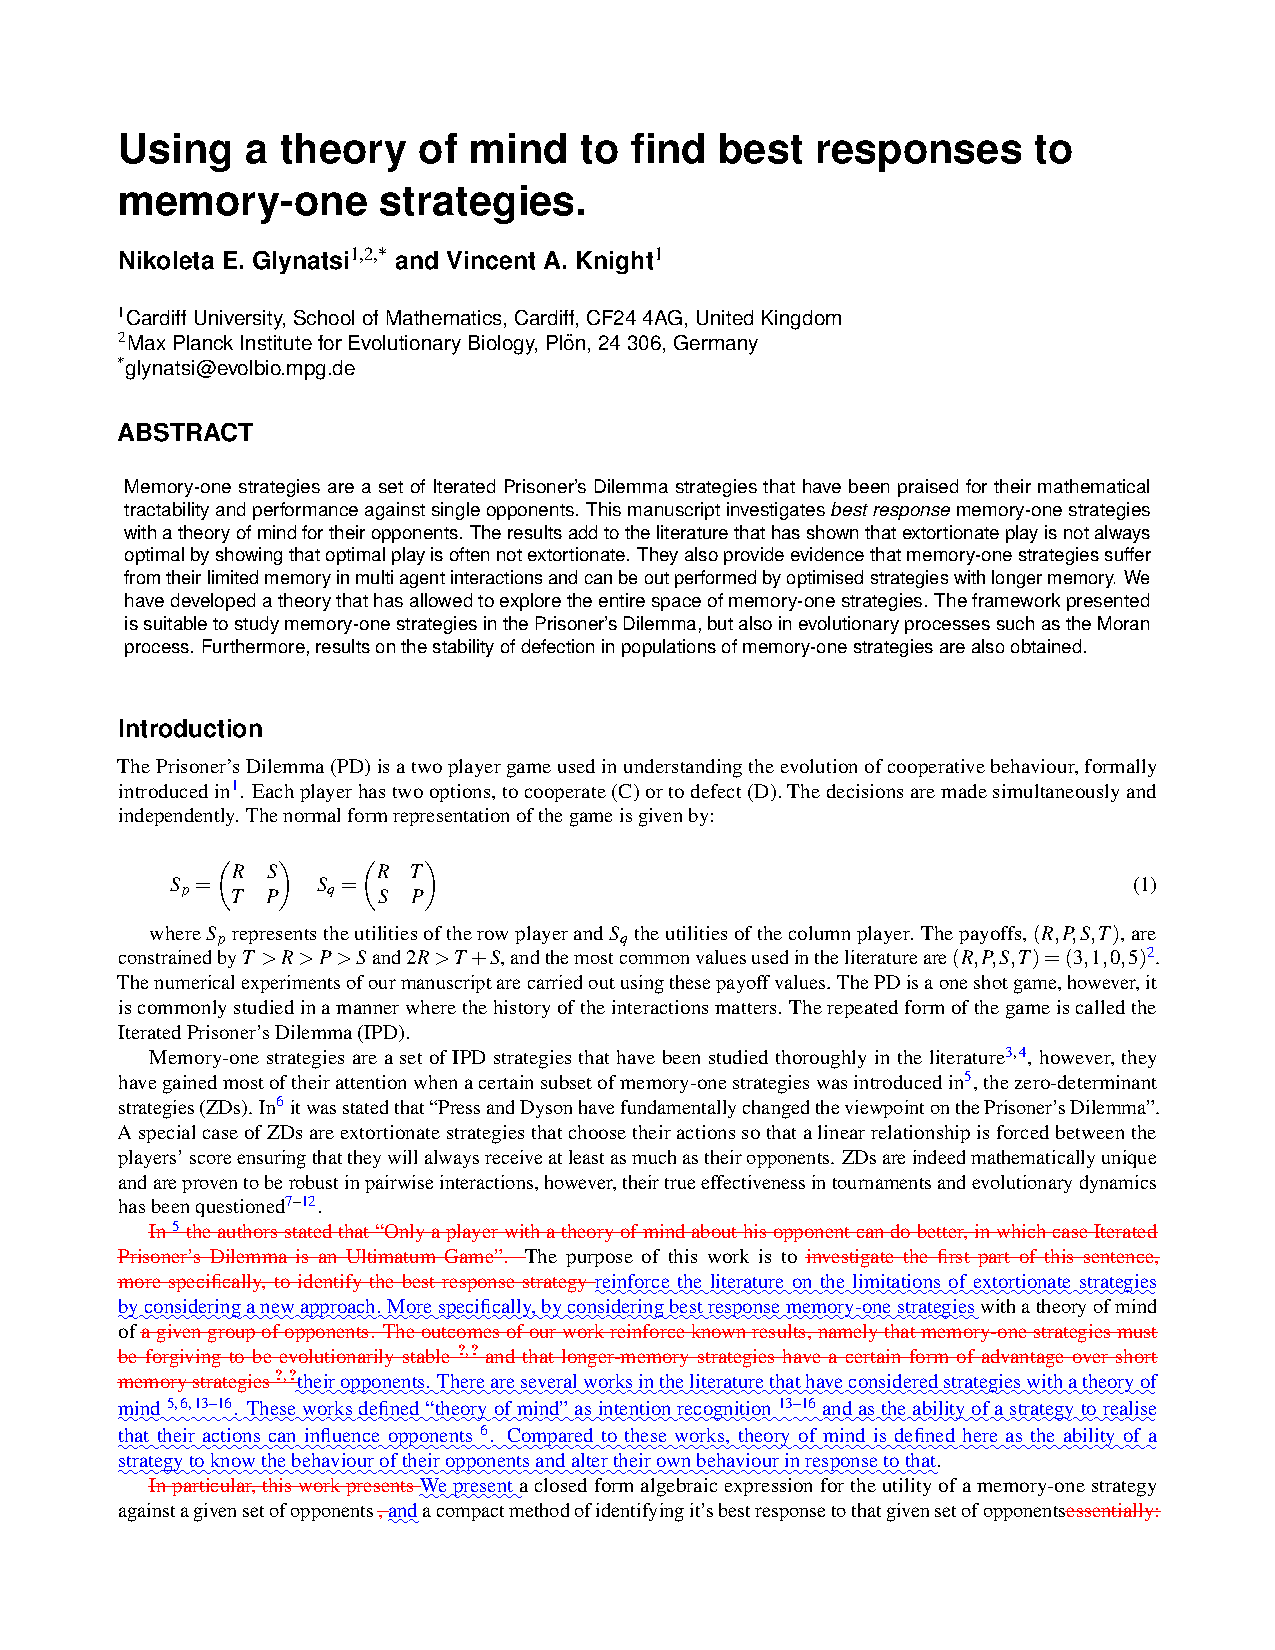
\includepdf[pages=-]{../diff.pdf}

\end{document}
